\chapter{Quantitative analysis of injection beam loss}\label{sec:Quantitative analysis of injection beam loss}

\section{Injection beam loss monitoring during the 2025c and 2026ab operations}

The beam current, injection efficiency, and injection beam losses are displayed on a Grafana dashboard, which can be accessed both from the collimator operation desk in the SuperKEKB control room and from personal computers via the web. 

\begin{figure}[htbp]
    \centering
    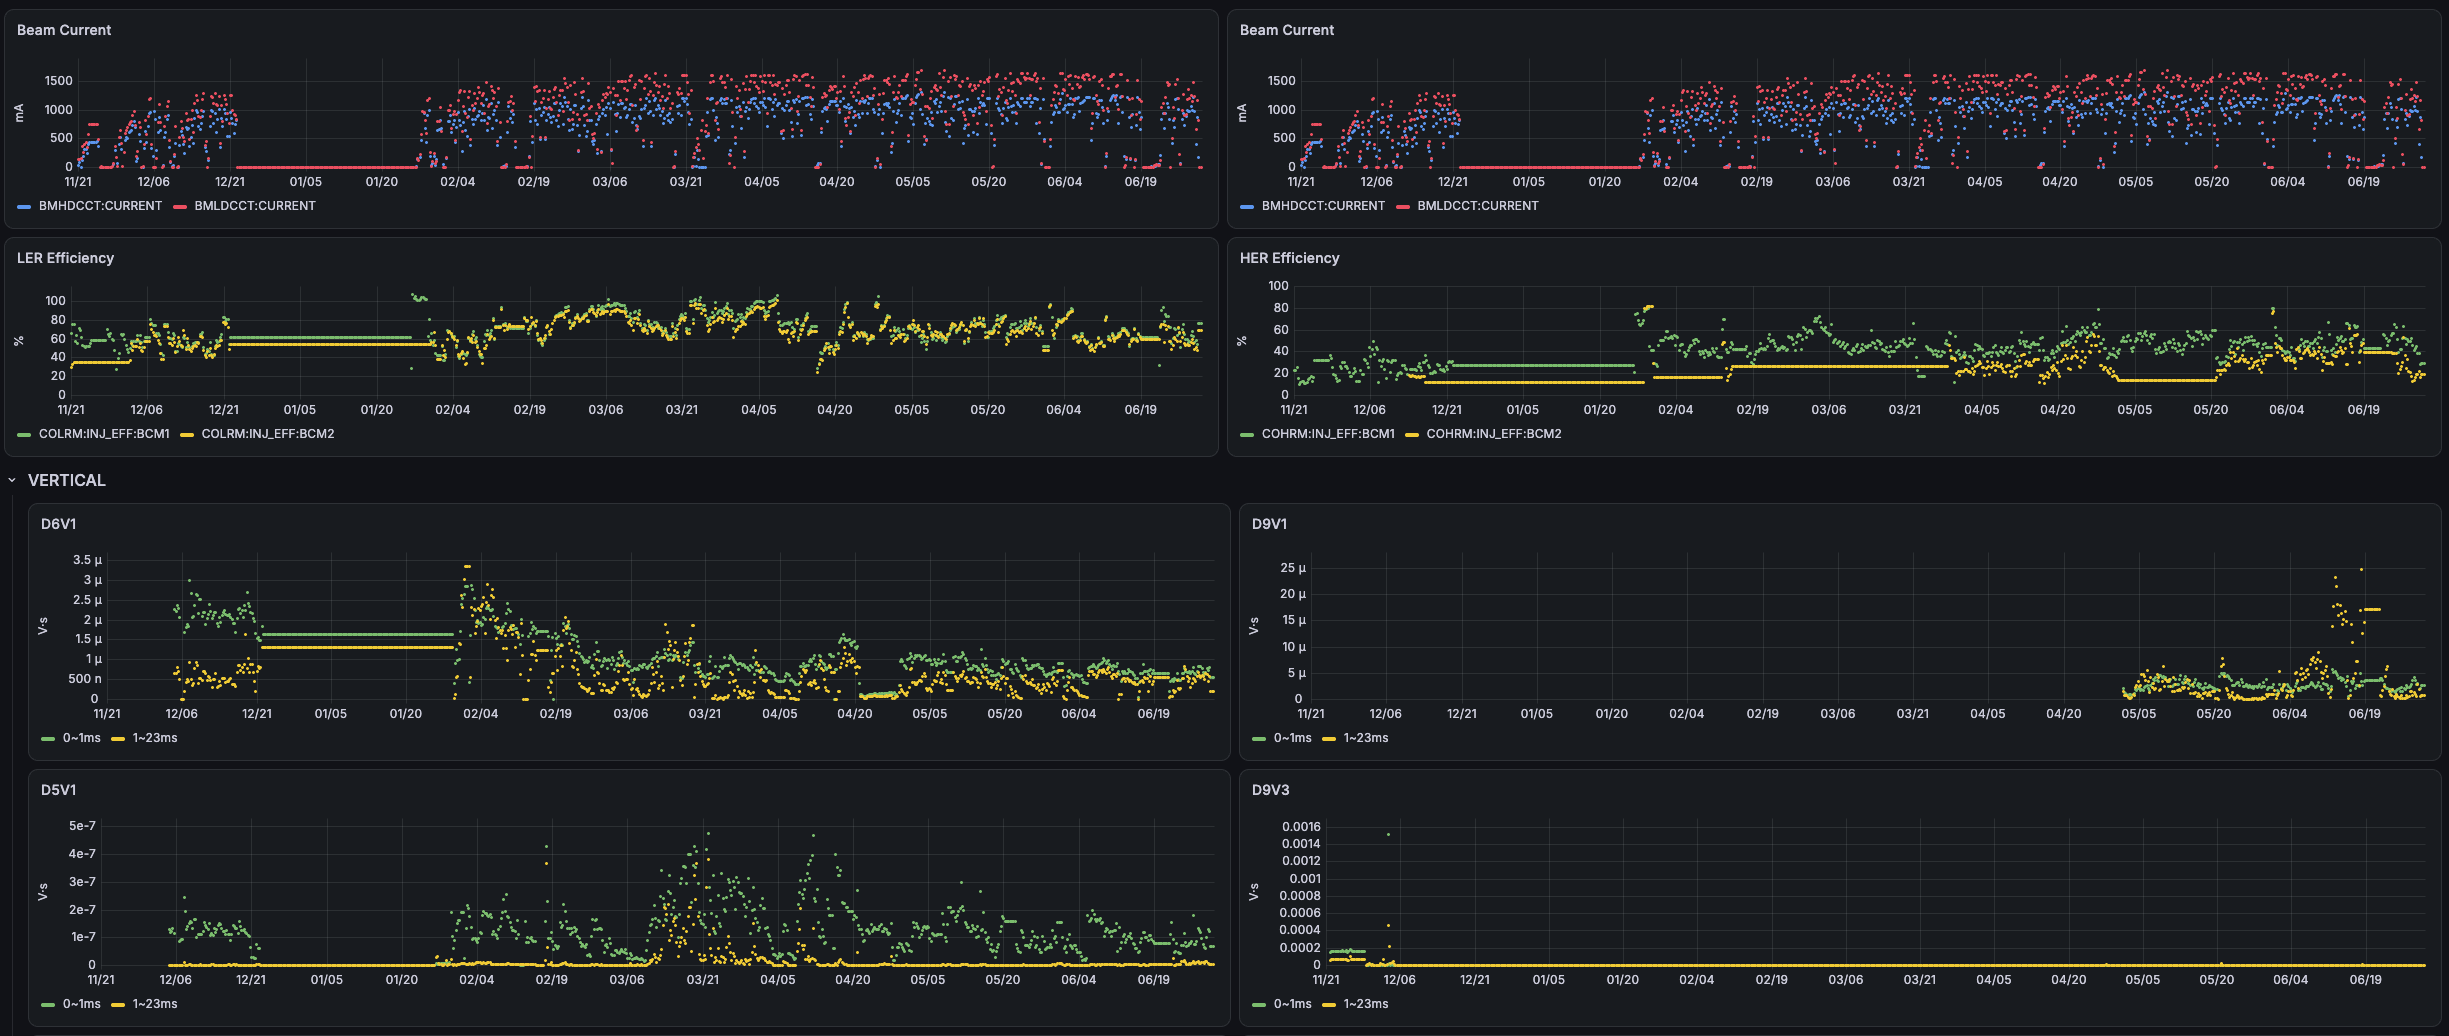
\includegraphics[width=1.0\columnwidth]{Figures/C05_Quantitative_analysis/monitor01.png}\\[-1.0pt]
    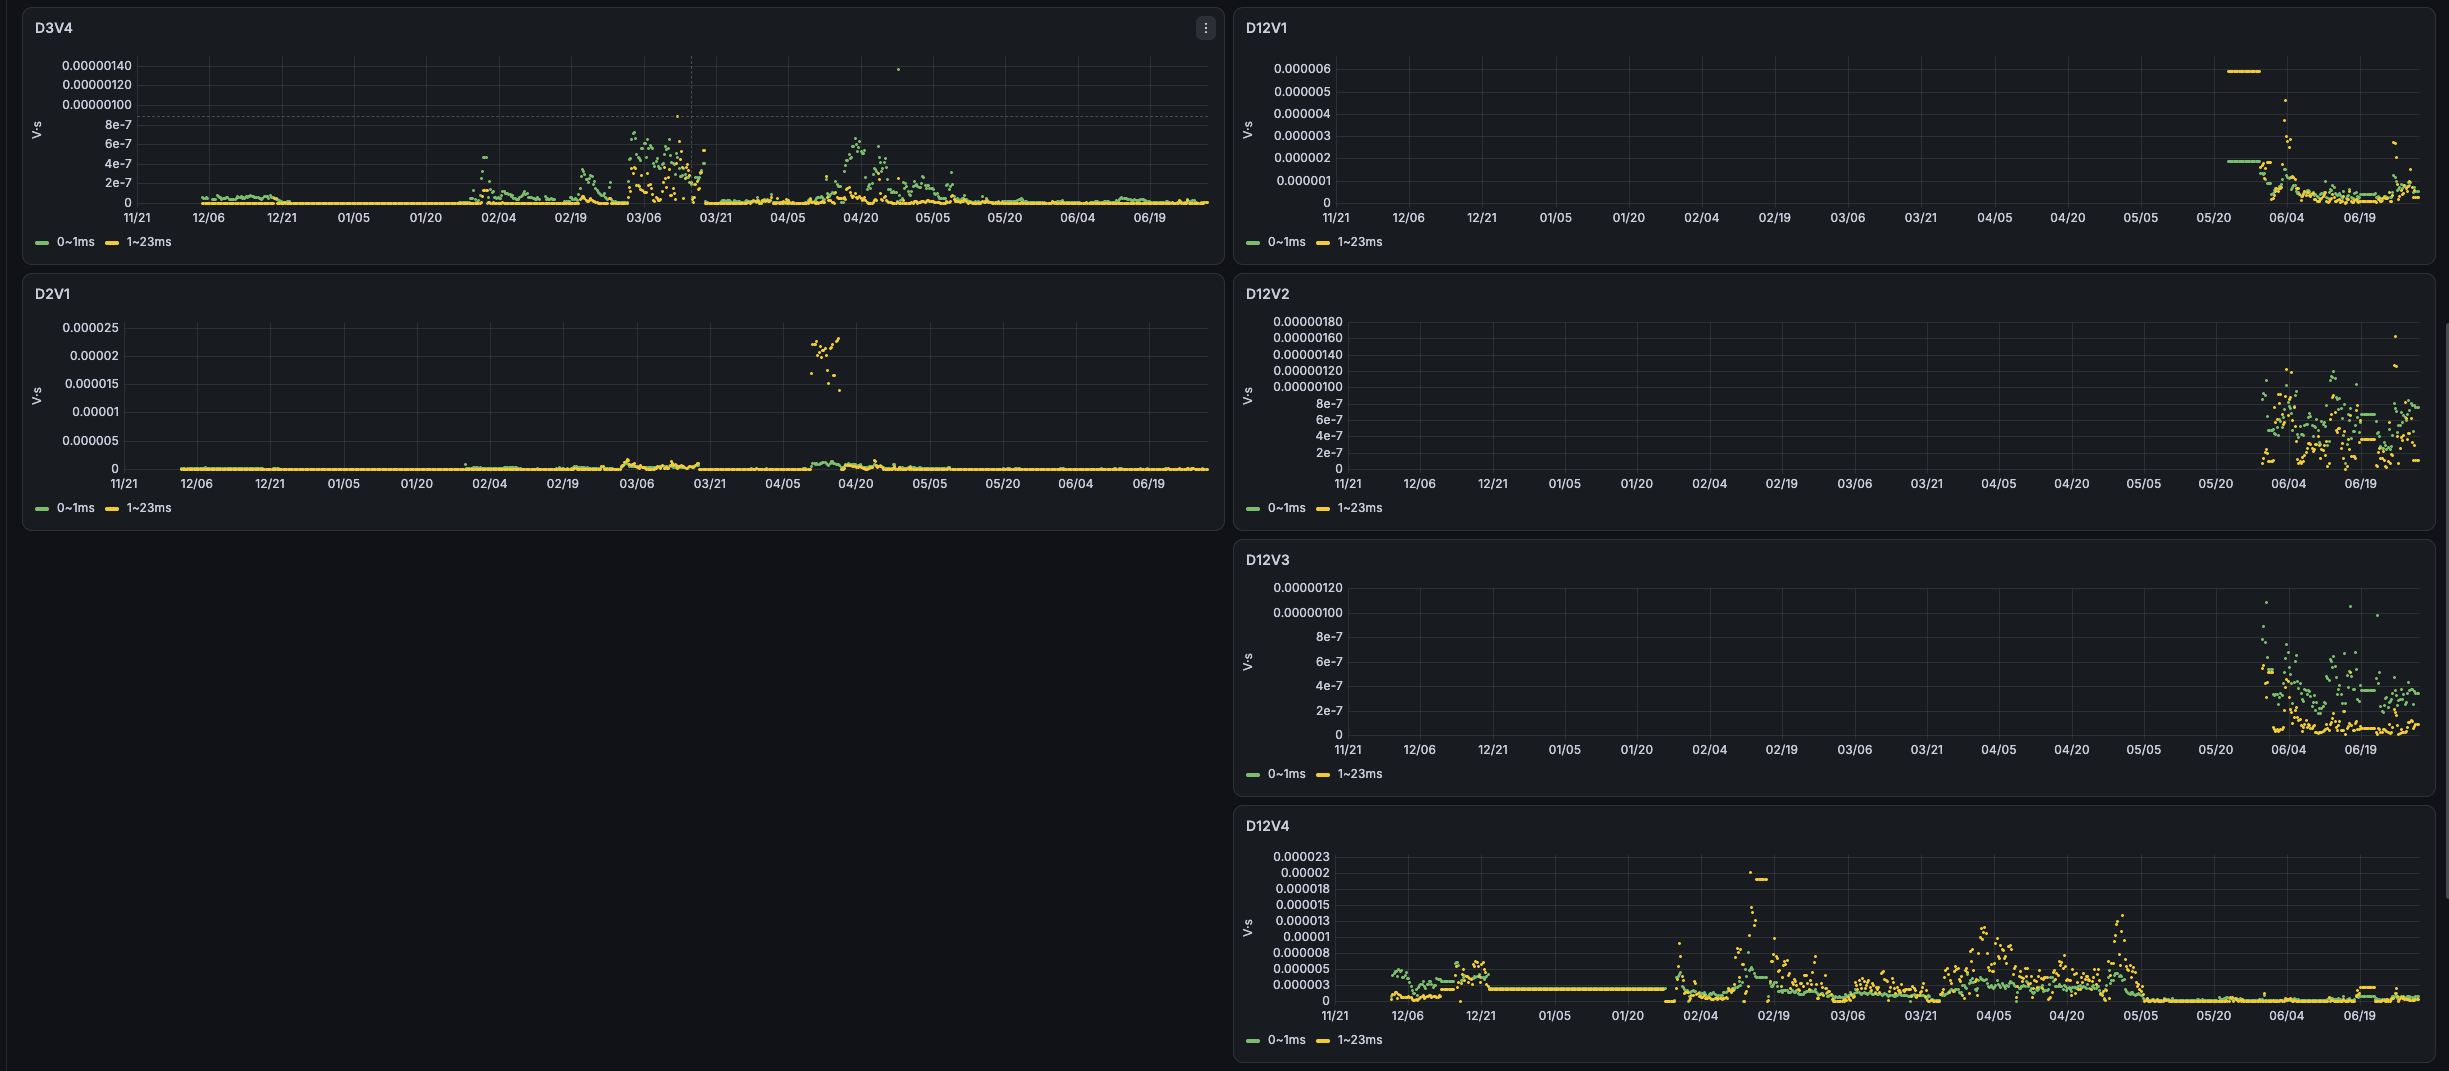
\includegraphics[width=1.0\columnwidth]{Figures/C05_Quantitative_analysis/monitor02.png}\\[-1.0pt]
    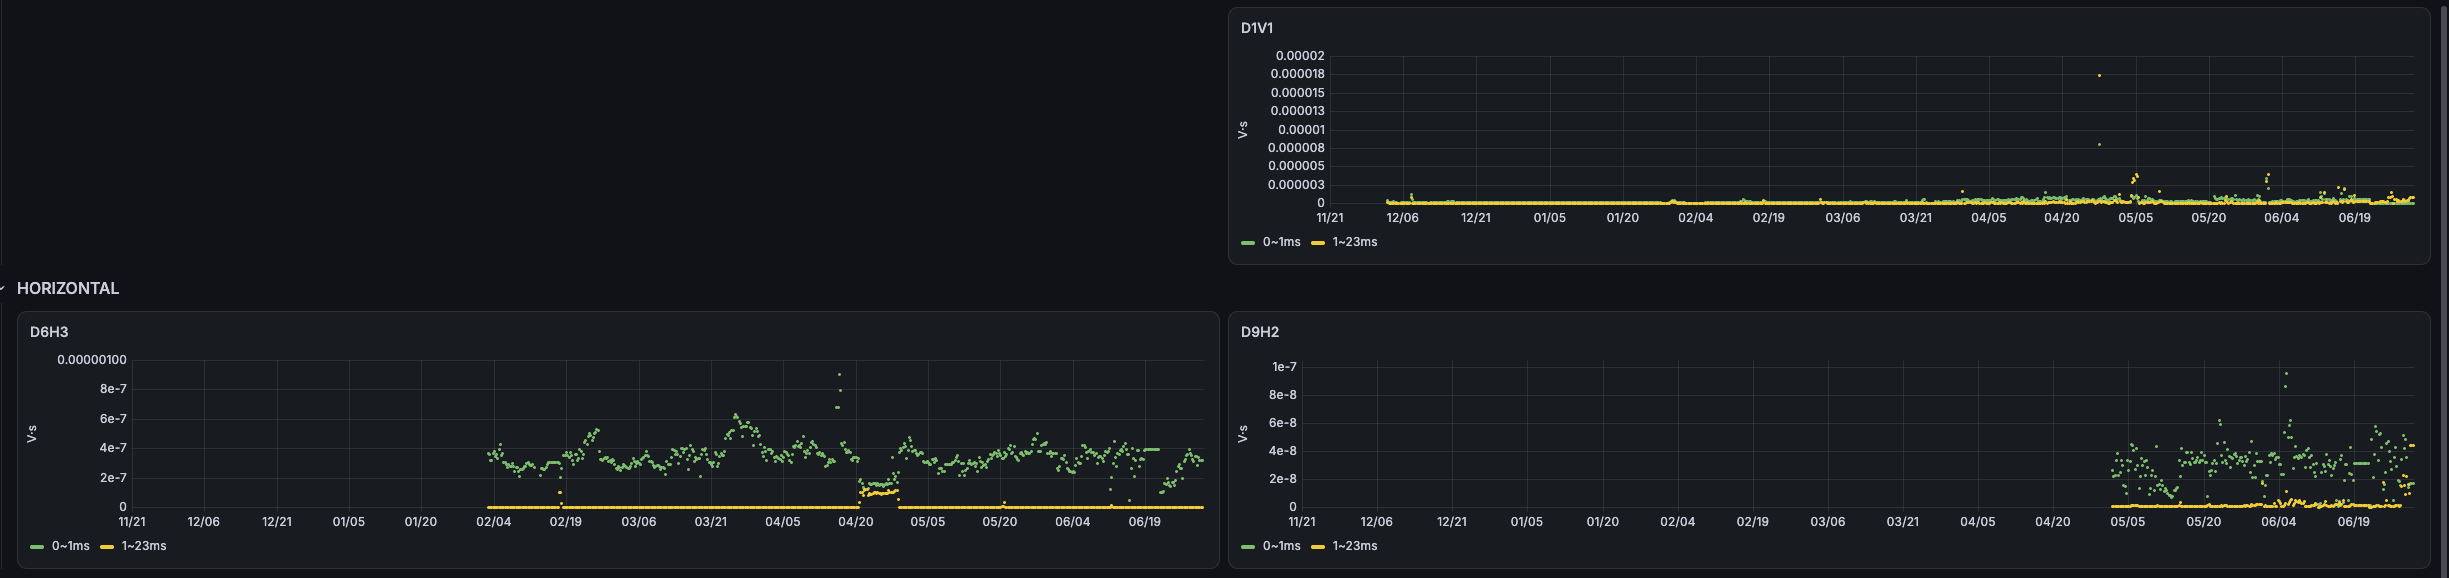
\includegraphics[width=1.0\columnwidth]{Figures/C05_Quantitative_analysis/monitor03.png}
    \caption{Injection beam loss monitoring during the 2025c and 2026ab operations. The left and right columns shows the LER and HER, respectively. The first row shows the beam current, and the second row shows the injection efficiencies. The remaining plots show the injection beam losses at the vertical and horizontal collimators, where the first losses i the first 1 ms after injection are shown in green and those after 1 ms shown in yellow.}
    \label{fig:Injection beam loss monitoring during the 2025c and 2026ab operations}
\end{figure}






\section{Collimator offset study}
\subsection{Motivation}
A collimator offset study measures the offset between the beam position coordinate and the collimator coordinate. By precisely determining this offset, the beam can be scraped symmetrically from both sides, enabling efficient collimation. When the center of the collimator coincides with the beam center, the beam loss at the collimator is minimized and the beam lifetime is maximized. The property is used to determine the offset. 

\subsection{Measurement procedure}
The procedure is as follows:

\begin{enumerate}
    \item \textbf{Move both collimator jaws while keeping the jaw gap constant:}
    Both jaws are moved in the same direction, typically in steps of 50 $\mu \mathrm{m} $. 

    \item \textbf{Monitor the beam response:}
    If no significant response is observed, apply a beam bump to modify the beam orbit near the target collimator.
    
    \item \textbf{Fit the measured response:}
    The center position of the collimator jaws is plotted on the x-axis, and the measured value is plotted on the y-axis. The distribution is fitted with a quartic function, 
    \begin{equation}
        y = a(x - x_0)^2 + b (x - x_0) + c, 
    \end{equation}
    and the offset is determined from the vertex position $-x_0$.

\end{enumerate}

Traditionally, the beam lifetime is used as the beam response. In this study, we additionally used the injection beam loss as the response. Unlike the beam lifetime, it can be measured during injection without requiring a dedicated measurement period. 

\subsection{D02V1 collimator}
The collimator offset study for D02V1 was conducted on November 14, 2025. The offset obtained from the injection beam loss was $-183 \pm 5 \mu \mathrm{m}$, while that from the beam lifetime was $-219 \pm 8 \mu\mathrm{m}$. The difference is 36 $\mu \mathrm{m} $, which is smaller than step width of 50 $\mu \mathrm{m} $. However, it corresponds to about 3.8 $\sigma$ when the statistical uncertainties are added in quadrature. This indicates that the two results are not consistent within their statistical errors, and that a systematic uncertainty of at least a few tens on $\mu \mathrm{m} $ is present. Possible sources include the choice of the fit function and fit range, and the difference in the beam response used by the two methods. 

\begin{figure}[htbp]
    \centering
    \begin{minipage}{0.48\columnwidth}
        \centering
        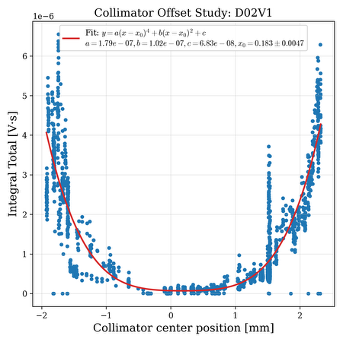
\includegraphics[width=\textwidth]{Figures/C05_Quantitative_analysis/Offset/D02V1.png}
    \end{minipage}
    \hfill
    \begin{minipage}{0.48\columnwidth}
        \centering
        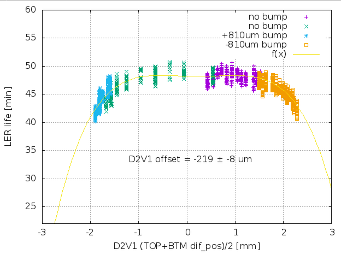
\includegraphics[width=\textwidth]{Figures/C05_Quantitative_analysis/Offset/D02V1_life.png}
    \end{minipage}
    \caption{Fitting results for D02V1: injection beam loss (left) and beam lifetime (right).}
    \label{fig:D02V1_fitting}
\end{figure}


\subsection{D03V4 collimator}
The collimator offset study for D03V4 was conducted on November 14, 2025. During this measurement, the oscilloscope configuration was  changed, resulting in incorrect response values. Figure~\ref{fig:D03V4_fitting} shows the results after excluding the affect data. As a result, the data points are concentrated on one side of the vertex
(roughly $-1.4$ to $+1.0\,\mathrm{mm}$), and the fit to the injection beam loss
did not converge to a satisfactory result:
$x_0 = -0.588 \pm 0.094\,\mathrm{mm}$.
In contrast, the fit to the beam lifetime gave a good result,
with an offset of $370 \pm 8\,\mu\mathrm{m}$.

\begin{figure}[htbp]
    \centering
    \begin{minipage}{0.48\columnwidth}
        \centering
        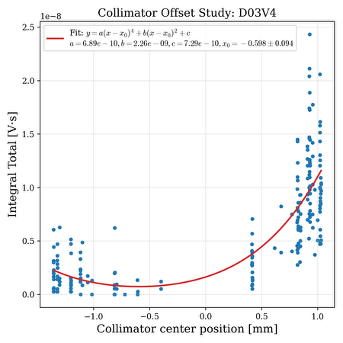
\includegraphics[width=\textwidth]{Figures/C05_Quantitative_analysis/Offset/D03V4.png}
    \end{minipage}
    \hfill
    \begin{minipage}{0.48\columnwidth}
        \centering
        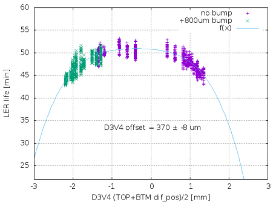
\includegraphics[width=\textwidth]{Figures/C05_Quantitative_analysis/Offset/D03V4_life.png}
    \end{minipage}
    \caption{Fitting results for D03V4: injection beam loss (left) and beam lifetime (right).}
    \label{fig:D03V4_fitting}
\end{figure}



\subsection{D01V1 collimator}
The collimator offset study for D01V1 was conducted on January 29, 2026. No significant response was observed in the beam lifetime, because no effective magnet was available to create a beam bump and modify the beam orbit near the D01V1 collimator. In contrast, a significant response was observed in the injection beam loss(Figure~\ref{fig:D01V1_fitting}), so the fit could be performed and the offset was determined to be $x_0 = -0.353 \pm 0.008\,\mathrm{mm}$. This offset was then adopted as the actual collimator setting. These results suggest that the injection beam loss can be used for the collimator offset study even in a case when beam lifetime shows no significant response. 


\begin{figure}[htbp]
    \centering
    \begin{minipage}{0.48\columnwidth}
        \centering
        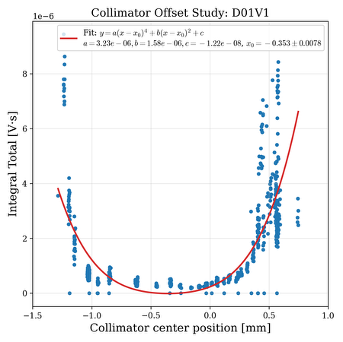
\includegraphics[width=\textwidth]{Figures/C05_Quantitative_analysis/Offset/D01V1.png}
    \end{minipage}
    \hfill
    \begin{minipage}{0.48\columnwidth}
        \centering
        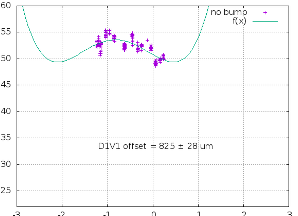
\includegraphics[width=\textwidth]{Figures/C05_Quantitative_analysis/Offset/D01V1_life.png}
    \end{minipage}
    \caption{Fitting results for D01V1: injection beam loss (left) and beam lifetime (right).}
    \label{fig:D01V1_fitting}
\end{figure}

\section{Temporal structure analysis}
\subsection{Purpose and principle of the FFT analysis}
The pulse-integral signal of each collimator loss monitor records the injection beam loss turn by turn. Its temporal structure contains information on the particle motion that causes the loss: a loss modulated at the betatron frequency indicates that betatron oscillation of the injected beam is responsible, whereas modulation at the synchrotron frequency indicates longitudinal motion. A Fast Fourier Transform (FFT) of this signal separates these contributions in the frequency domain, so that the origin of the injection beam loss can be identified and used as beam-diagnosis information. 

\subsection{Tunes and their observed frequencies}
A circular collider has three tune parameters: the horizontal betatron tune $Q_x$, the vertical betatron tune $Q_y$, and the synchrotron tune $Q_s$. Each tunes are the number of oscillations per revolution and is written as the sum of an integer part and fractional part. Only fractional part is relevant here, as explained below. The tunes are coupled to each other through effects such as $x$--$y$ coupling and synchro-betatron coupling. 


We performed FFT analysis on the Pulse Integral signal of the injection beam loss detected at each collimator. To avoid the effect of large injection beam oscillation, we selected after 1 ms signal. The time resolution of pulse integral signal is about 10 us that corresponds to the time revolution of SuperKEKB, so the nichist frequency is about 50,000 Hz. If the fluctional part of tune exceed 0.5, a reversal occurs, 1-Q. 

The pulse-integral signal provides one value per revolution, so the sampling frequency equals the revolution frequency $\frev = 1/T_{\mathrm{rev}}$, with $T_{\mathrm{rev}} = 10.0614\,\mu\mathrm{s}$ for the LER ($\frev \simeq 99.4\,\mathrm{kHz}$). An oscillation with tune $Q = n + \nu$ ($n$ integer, $0 \le \nu < 1$) therefore appears at the frequency $\nu\,\frev$ in the spectrum. Since the spectrum of a real signal is only defined up to the Nyquist frequency $\frev/2 \simeq 49.7\,\mathrm{kHz}$, a fractional part $\nu > 0.5$ is folded back (aliased) and observed at $(1-\nu)\, \frev$. The expected frequencies of the LER tunes are summarized in Table~\ref{tab:oscillation_frequency}. For $Q_s$ only the magnitude matters, because the spectrum does not distinguish the sign of the frequency. 

\begin{table}[htbp]
    \centering
    \begin{tabular}{lcccc}
        \hline
        Tune & Value & Fractional part $\nu$ & Observed fraction & Frequency [Hz] \\
        \hline
        $Q_x$ (LER) & $44.538$  & $0.538$   & $1-\nu = 0.462$  & $45920$ \\
        $Q_y$ (LER) & $46.588$  & $0.588$   & $1-\nu = 0.412$  & $40950$ \\
        $Q_s$ (LER) & $-0.0233$ & $0.0233$  & $|\nu| = 0.0233$ & $2320$  \\
        \hline
    \end{tabular}
    \caption{Number of oscillations per turn and the corresponding frequencies in the spectrum.
    The frequency is the observed fraction multiplied by $\frev = 1/(10.0614\,\mu\mathrm{s})$.
    The values were measured on {date / machine condition}.}
    \label{tab:oscillation_frequency}
\end{table}


\subsection{Analysis method}
We performed the FFT on the pulse-integral signal of the injection beam loss detected at each collimator. To avoid the effect of the large injectino beam oscillation immediately after injection, only the signal later thajn 1~ms after injection was used. The time resolution of the pulse-integral singal is about $10\,\mu\mathrm{s}$, which corresponds to the revolution time of superKEKB, so that Nyquist frequency is about $50\,\mathrm{kHz}$. The frequency resolution is determined by the length $T$ of the analyzed signal, $\Delta f = 1/T$. The typical signal length is a few milliseconds, corresponding to a few hundred turns, so the frequency resolution is about several hundred Hz. 

\subsection{Spectrum of the injection beam loss}

\begin{figure}[htbp]
    \centering
    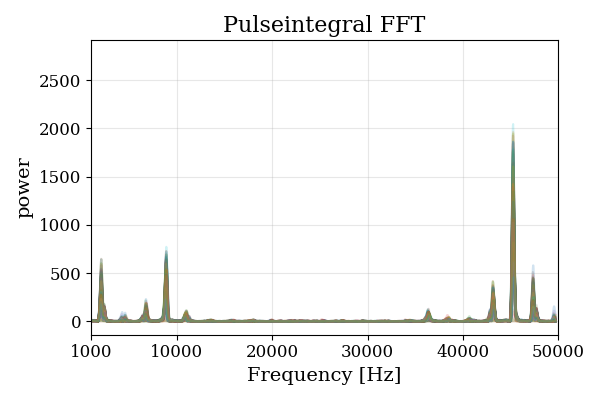
\includegraphics[width=0.6\columnwidth]{Figures/C05_Quantitative_analysis/FFT/typical_spectrum.png}
    \caption{Typical spectrum of injection beam loss for LER, detected at D6V1. The dominant peak at about 46\,kHz is the horizontal betatron tune $Q_x$, with the synchro-betatron sidebands $Q_x \pm Q_s$ on both sides. The peak at the left edge corresponds to $Q_s$. }
    \label{fig:typical spectrum}
\end{figure}

Figure~\ref{fig:typical spectrum} shows a typical spectrum. The dominant peak at about 46\,kHz is attributed to the horizontal betatron tune. The sidebands of this peak are attributed to synchro-betatron coupling, $Qx \pm Qs$. Their expected positions are $45.92 \pm 2.32\,\mathrm{kHz}$, i.e.\ $43.6\,\mathrm{kHz}$ and $48.2\,\mathrm{kHz}$, which agree with the observed side  peaks. The peak at the left edge is attributed to the synchrotron tune. These peaks agree with the measured tunes in Table~\ref{tab:oscillation_frequency} within the resolution of the analysis. The peak corresponds to $Q_y$ ($40.95\,\mathrm{kHz}$) does not appear in the spectrum. 

Further peaks are visible at around 9\,kHz, and 36\,kHz. These are probably higher-order components of the horizontal tune: the fractional part of $2Q_x$ gives $\simeq 7.6\,\mathrm{kHz}$ and that of $3Q_x$ gives $\simeq 38.4\,\mathrm{kHz}$, close to the observed positions. 

\subsection{Tune scan}
To confirm the origin of these peaks, horizontal and vertical tune scans were conducted in parallel with the high bunch current study (Section~\ref{sec:high_bunch_current} ). The measurement was performed under two conditions: single beam and collision. In each scan, one tune was changed in steps while the injection beam loss spectrum was recorded. The results are shown as a map of the spectrum as a function of the measured tune (Figures~\ref{fig:LER tune X scan} and \ref{fig:LER tune Y scan}. 

If a peak originates from $Q_x$, its frequency should follow  $f  = (1-\nu_x)\, \frev$ and move by $\Delta f = -\frev\,\Delta\nu_x$. For the scan range $\Delta\nu_x = 0.030$ (44.525--44.555) this corresponds to a shift of about $-3.0\,\mathrm{kHz}$. The $Q_s$ peak should stay at a fixed frequency, because $Q_s$ is not changed by the scan. 

\begin{figure}[htbp]
    \centering
    \begin{minipage}{0.48\columnwidth}
        \centering
        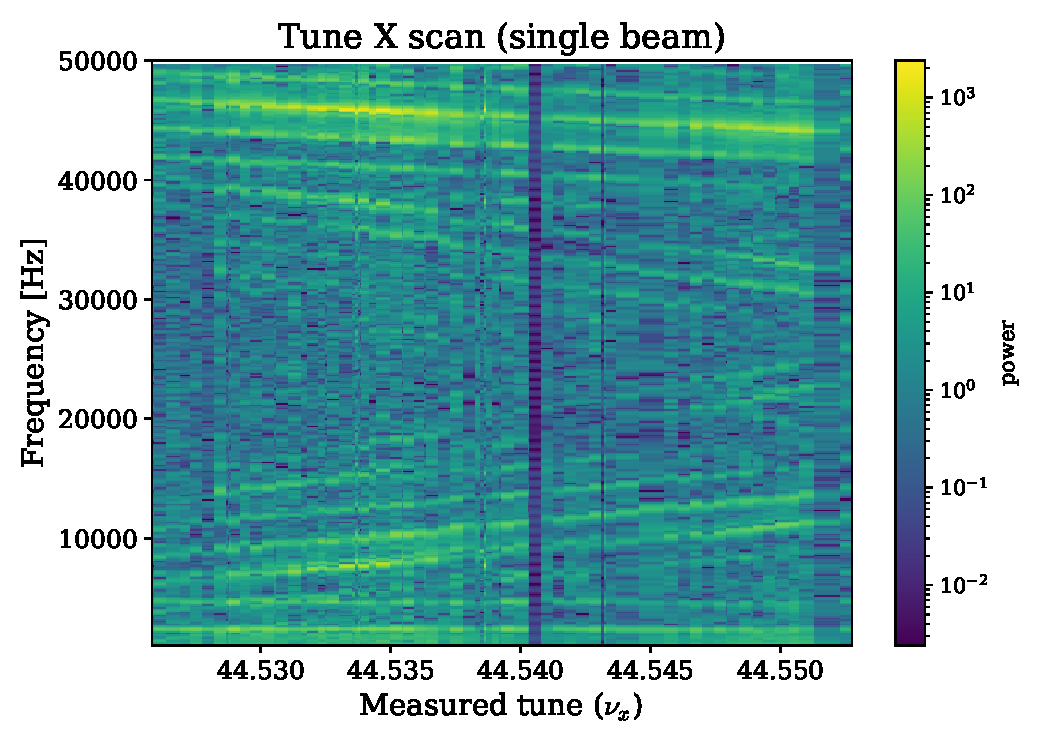
\includegraphics[width=\textwidth]{Figures/C05_Quantitative_analysis/FFT/2026-06-16_tuneX_single_beam_map.pdf}
    \end{minipage}
    \hfill
    \begin{minipage}{0.48\columnwidth}
        \centering
        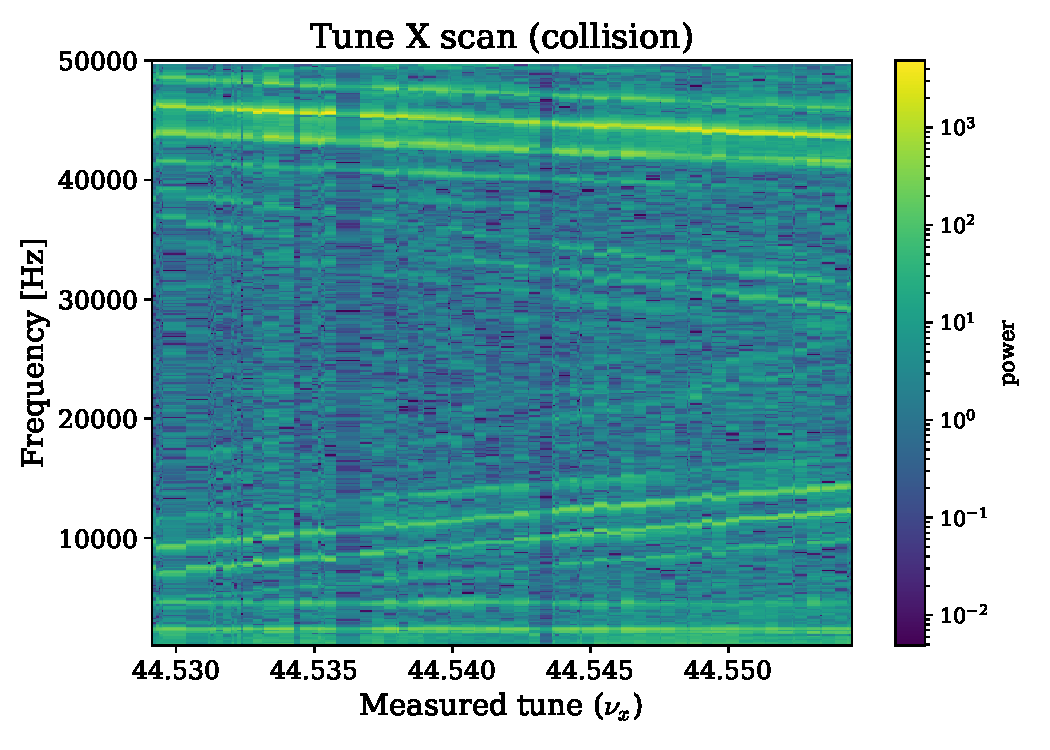
\includegraphics[width=\textwidth]{Figures/C05_Quantitative_analysis/FFT/2026-06-16_tuneX_collision_map.pdf}
    \end{minipage}
    \caption{LER tune $X$ scan for single beam (left) and with collision (right). The color shows the FFT power of the injection beam loss. the dominant peak moves from about 46.5\,kHz to 44.5\,kHz as the horizontal tune increases.}
    \label{fig:LER tune X scan}
\end{figure}

Figure~\ref{fig:LER tune X scan} shows the horizontal tune scan. The dominant peak moves downward by about 3\,kHz over the scan range, which agrees with the expected shift $-\frev\,\Delta\nu_x \simeq -3.0\,\mathrm{kHz}$.
The sidebands shift in the same direction, and the peak corresponding to $Q_s$ does not shift.
These behaviors are the same in single beam and in collision.

\begin{figure}[htbp]
    \centering
    \begin{minipage}{0.48\columnwidth}
        \centering
        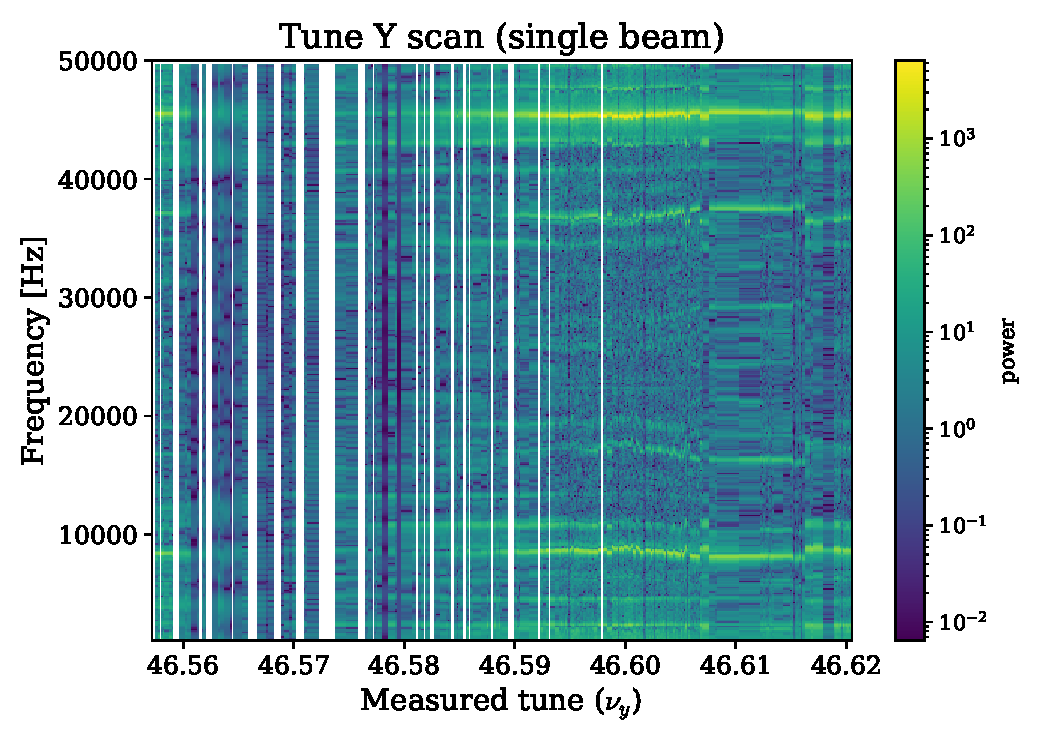
\includegraphics[width=\textwidth]{Figures/C05_Quantitative_analysis/FFT/2026-06-16_tuneY_single_beam_map.pdf}
    \end{minipage}
    \hfill
    \begin{minipage}{0.48\columnwidth}
        \centering
        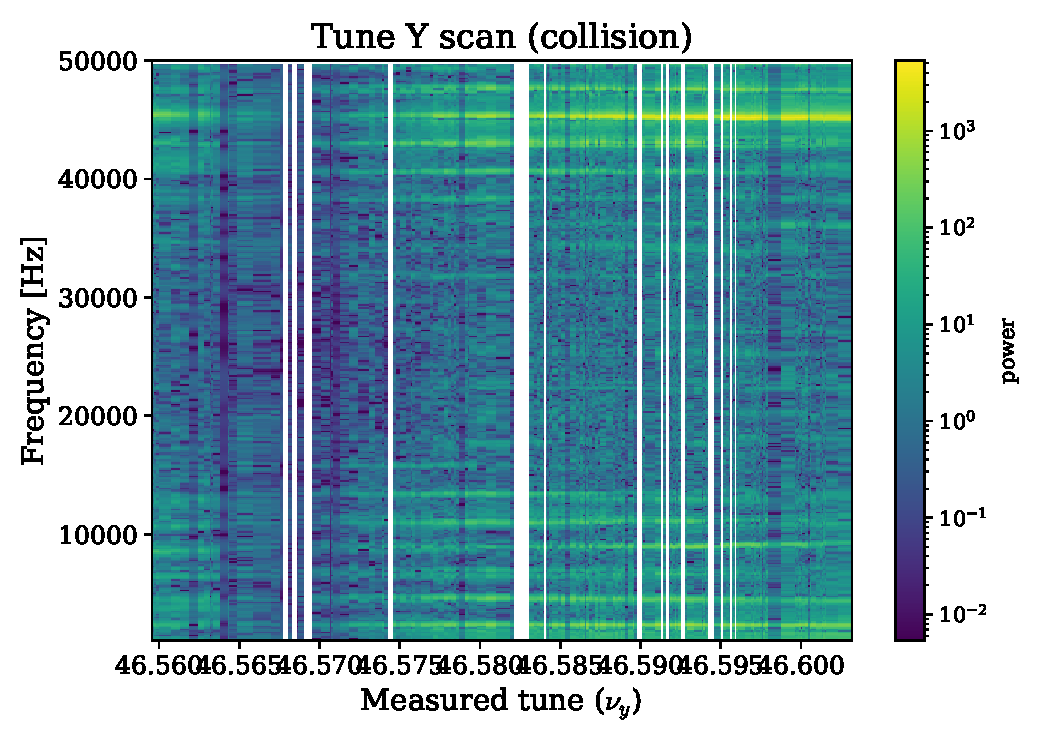
\includegraphics[width=\textwidth]{Figures/C05_Quantitative_analysis/FFT/2026-06-16_tuneY_collision_map.pdf}
    \end{minipage}
    \caption{LER tune $Y$ scan for single beam (left) and with collision (right).In the section where some peak positions vary, the horizontal tune also changed because of the machine operation.}
    \label{fig:LER tune Y scan }
\end{figure}

Figure~\ref{fig:LER tune Y scan} shows the vertical tune scan. The dominant peak stays at about 46\,kHz while $\nu_y$ is varied, so it does not originate from the vertical tune. In the section where some peak positions vary, the horizontal tune changed because of the machine operation, and the peaks that move there are therefore related to $Q_x$. 

It is worth noting that the horizontal oscillation is observed at the vertical collimator. 





\section{High bunch current study}
\newcommand{\Iinj}{I_{\mathrm{inj}}}
\newcommand{\Iopp}{I_{\mathrm{opp}}}
\subsection{Motivation}

Future operation of SuperKEKB requires higher bunch currents, which strengthen the beam-beam effect and may degrade the injection. Injected bunches that are lost near the interaction region (IR) can also increase the background of the detector. The high bunch current study was therefore performed to examine the effect of high bunch current on the injection without taking risks of high-current collision operation, such as a large background at the IR. Using the injection beam loss monitors installed at the collimators, we measured how the injection beam loss and the injection efficiency depend on the bunch current in each ring, with single beam and with collision. Two bunch currents are important in this study:
the bunch current of the bucket into which the new bunch is injected, and, in collision, the bunch current of the opposite-ring bunch that collides with the injected bunch at the IR. The letter is used to assess the beam-beam effect on the injected beam. 

\subsection{Measurement conditions}

The study was performed on June 16, 2026, with 393 bunches in each ring. The bunch current was increased step by step in the range of approximately 0.1 -1.0 mA, in the LER and 0.1 - 0.7 mA in the HER. The beam currents and the other quantities during the whole study are shown in FIG.~\ref{fig:HBC_study_config}, where the periods used in the analysis are shaded. The tune scans of Section~\ref{sec:tune_scan} were performed in parallel with this study.



\begin{figure}[htbp]
    \centering
    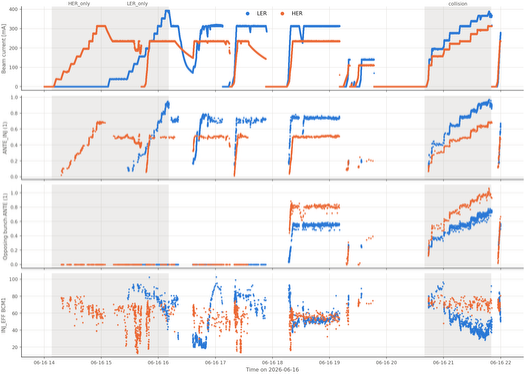
\includegraphics[width=0.8\columnwidth]{Figures/C05_Quantitative_analysis/HBCstudy/config.png}
    \caption{Time evolution of the study on June 16, 2026. From top to bottom: LER (blue) and HER (orange) beam current;
    bunch current of the bucket into which the bunch is injected ($\Iinj$);
    bunch current of the opposite-ring bunch that collides with the injected bunch ($\Iopp$);
    injection efficiency. Colors denote the ring into which the beam is injected.
    The shaded periods (HER only, LER only, collision) are used in the analysis.}
    \label{fig:HBC_study_config}
\end{figure}


\subsection{Definitions and analysis method}
\paragraph{Bunch currents.}
We use the following two quantities, both measured just before the injection in units of mA.
\begin{itemize}
    \item $\Iinj$ (\texttt{ANTE\_INJ}): the bunch current already stored in the bucket into which the injected bunch is put.
    \item $\Iopp$ (\texttt{ANTE\_(opposite ring)}): the bunch current of the opposite-ring bunch that collides at the IR with the injected bunch. For the LER injection it is the HER bunch current, and for the HER injection it is the LER bunch current.
\end{itemize}
In single beam, $\Iopp$ is not defined because the injected bunch does not collide with any bunch. 

\paragraph{Single beam and collision.}
A period is called "single beam" when the beams do not collide, even if the opposite ring stores beam. A period is called "collision" when the two rings collide at the IR. 

\paragraph{Injection beam loss and efficiency.}
The injection beam loss is the total pulse integral. The injection efficiency is obtained from the bunch current monitor (BCM). In the double-bunch injection, two bunches are injected, and the efficiencies 1 and 2 are those of the first and the second injected bunch, respectively. 

\paragraph{Analysis.}
Each injection is one data point. The data are binned in $\Iinj$ or $\Iopp$, and the mean and the standard deviation in each bin are plotted. The number of data points $N$ is shown in each panel. As a measure of the dependence, the Pearson correlation coefficient $r$ is used. Since several curves are not monotonic, is only a rough measure of the trend. We use the loss monitors of the vertical collimators D2V1, D3V4, D5V1, and D6V1 in the LER, and those of D1V1, D9V1, D9H2 (the only horizontal collimator), D9V3, and D12V1 - D12V4 in the HER. 



\subsection{LER}

\begin{figure}[htbp]
    \centering
    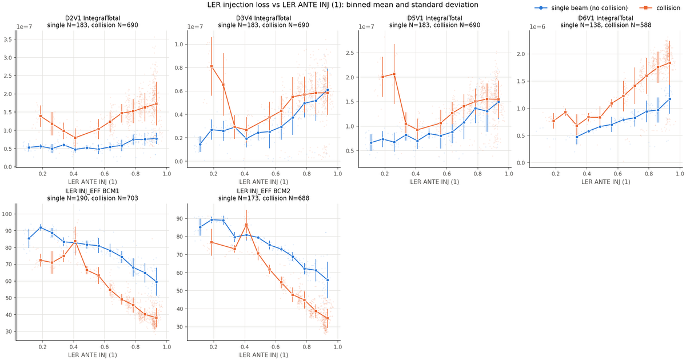
\includegraphics[width=0.8\columnwidth]{Figures/C05_Quantitative_analysis/HBCstudy/LER_ante_INJ.png}
    \caption{LER injection: dependence on the stored bunch current $\Iinj$ of the injected bucket.
    Upper panels: injection beam loss at each collimator.
    Lower panels: injection efficiency 1 and 2.
    Blue: single beam, orange: collision.}
    \label{fig:LER_ante_INJ}
\end{figure}


Figure~\ref{fig:LER_ante_INJ} shows the dependence on $\Iinj$. In single beam, the injection beam loss increases moderately with $\Iinj$, and the injection efficiency decreases from approximately 90\% to 60\%. With collision, the injection beam loss is larger than in single beam at D2V1 and D6V1 over the whole range. At D3V4 and D5V1, it is larger at low $\Iinj$ and approaches the single-beam value above approximately 0.6\,mA. The efficiency with collision is lower than that in single beam over most of the range (approximately 70\% to 35\%), and it decreases as $\Iinj$ increases. With collision, the injection beam loss and the injection efficiency show a bend at $\Iinj \simeq 0.4$\,mA: the bend is seen only with collision.

\begin{figure}[htbp]
    \centering
    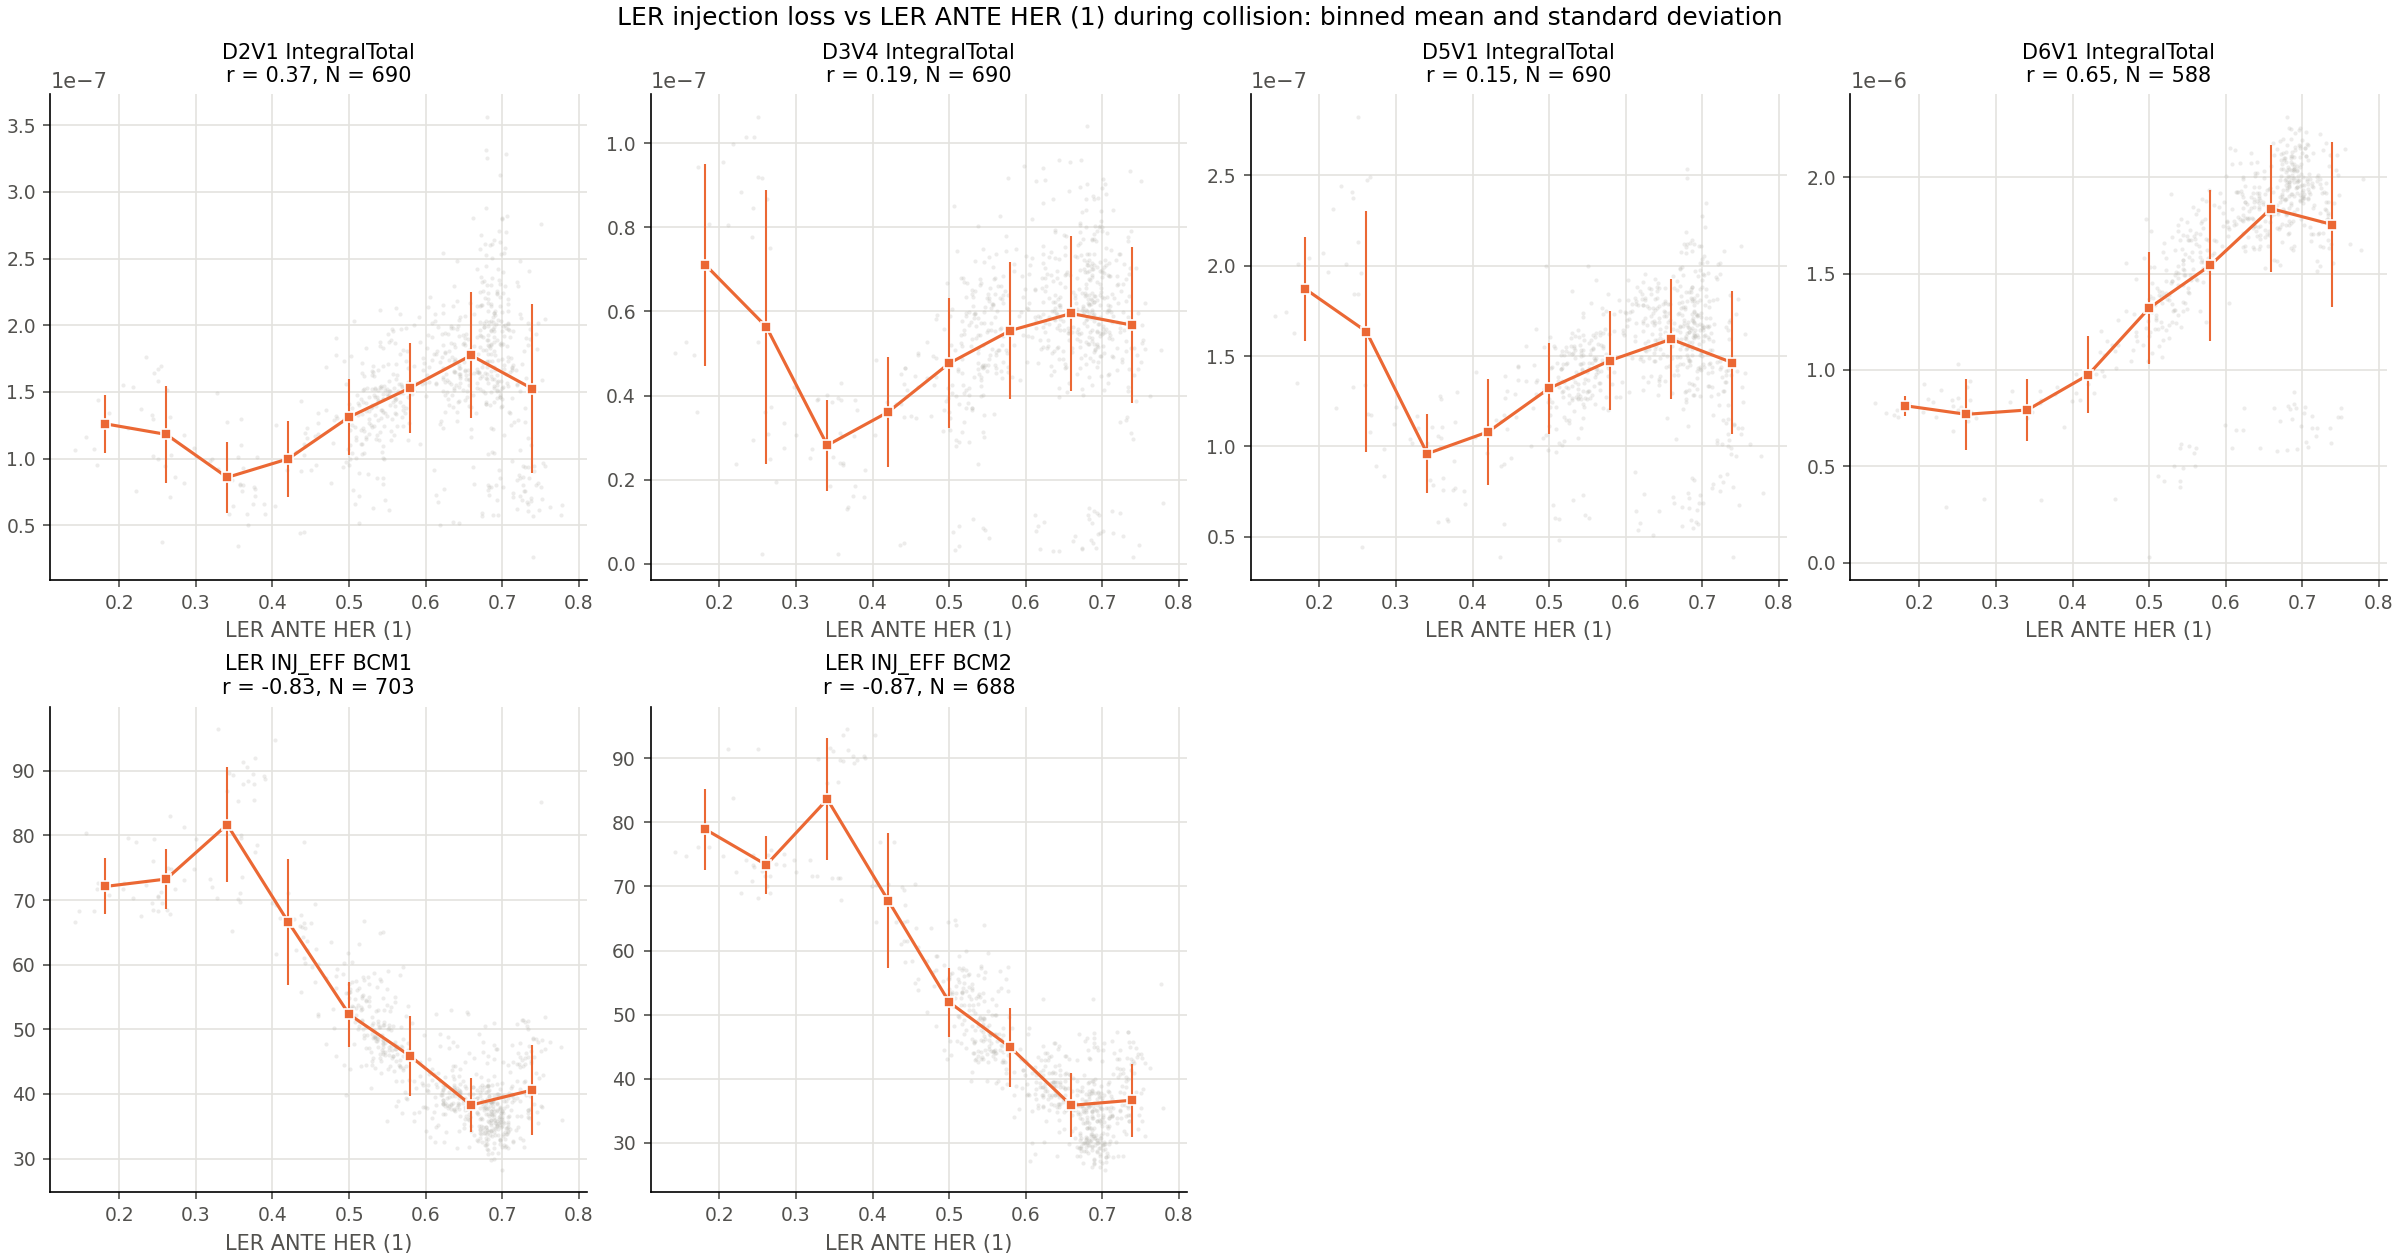
\includegraphics[width=0.8\columnwidth]{Figures/C05_Quantitative_analysis/HBCstudy/LER_ante_HER.png}
    \caption{LER injection with collision: dependence on the bunch current $\Iopp$ of the HER bunch that collides with the injected bunch.
    Upper panels: injection beam loss at each collimator.
    Lower panels: injection efficiency 1 and 2.}
    \label{fig:LER_ante_HER}
\end{figure}

Figure~\ref{fig:LER_ante_HER} shows the dependence on the colliding HER bunch current $\Iopp$. The injection beam loss increases with $\Iopp$ at all four collimators, with correlation coefficients of $r = 0.37$ (D2V1), $0.19$ (D3V4), $0.15$ (D5V1), and $0.65$ (D6V1). The correlation is strong only at D6V1. The injection efficiency decreases strongly with $\Iopp$ ($r = -0.83$ and $-0.87$ for efficiencies 1 and 2), from approximately 80\% at $\Iopp \simeq 0.45$\,mA to approximately 35\% at 0.7\,mA. The loss at D2V1, D3V4, and D5V1 also has a minimum around 0.4\,mA, as in Fig.~\ref{fig:LER_ante_INJ}.


\subsection{HER}


\begin{figure}[htbp]
    \centering
    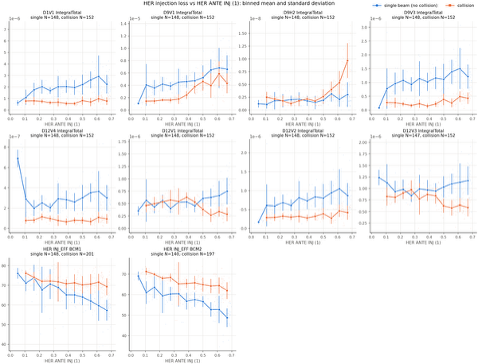
\includegraphics[width=0.8\columnwidth]{Figures/C05_Quantitative_analysis/HBCstudy/HER_ante_INJ.png}
    \caption{HER injection: dependence on the stored bunch current $\Iinj$ of the injected bucket.
    Upper panels: injection beam loss at each collimator.
    Lower panels: injection efficiency 1 and 2.
    Blue: single beam, orange: collision.}
    \label{fig:HER_ante_INJ}
\end{figure}

 
Figure~\ref{fig:HER_ante_INJ} shows the dependence on $\Iinj$.
In contrast to the LER, the injection beam loss in single beam is larger than that with collision at most collimators, and it increases with $\Iinj$.
The injection efficiency is higher with collision than in single beam, and in single beam it decreases with $\Iinj$.
D9H2, the only horizontal collimator, is an exception: with collision its loss increases rapidly at high $\Iinj$
(above approximately 0.5\,mA) and exceeds the single-beam value.

\begin{figure}[htbp]
    \centering
    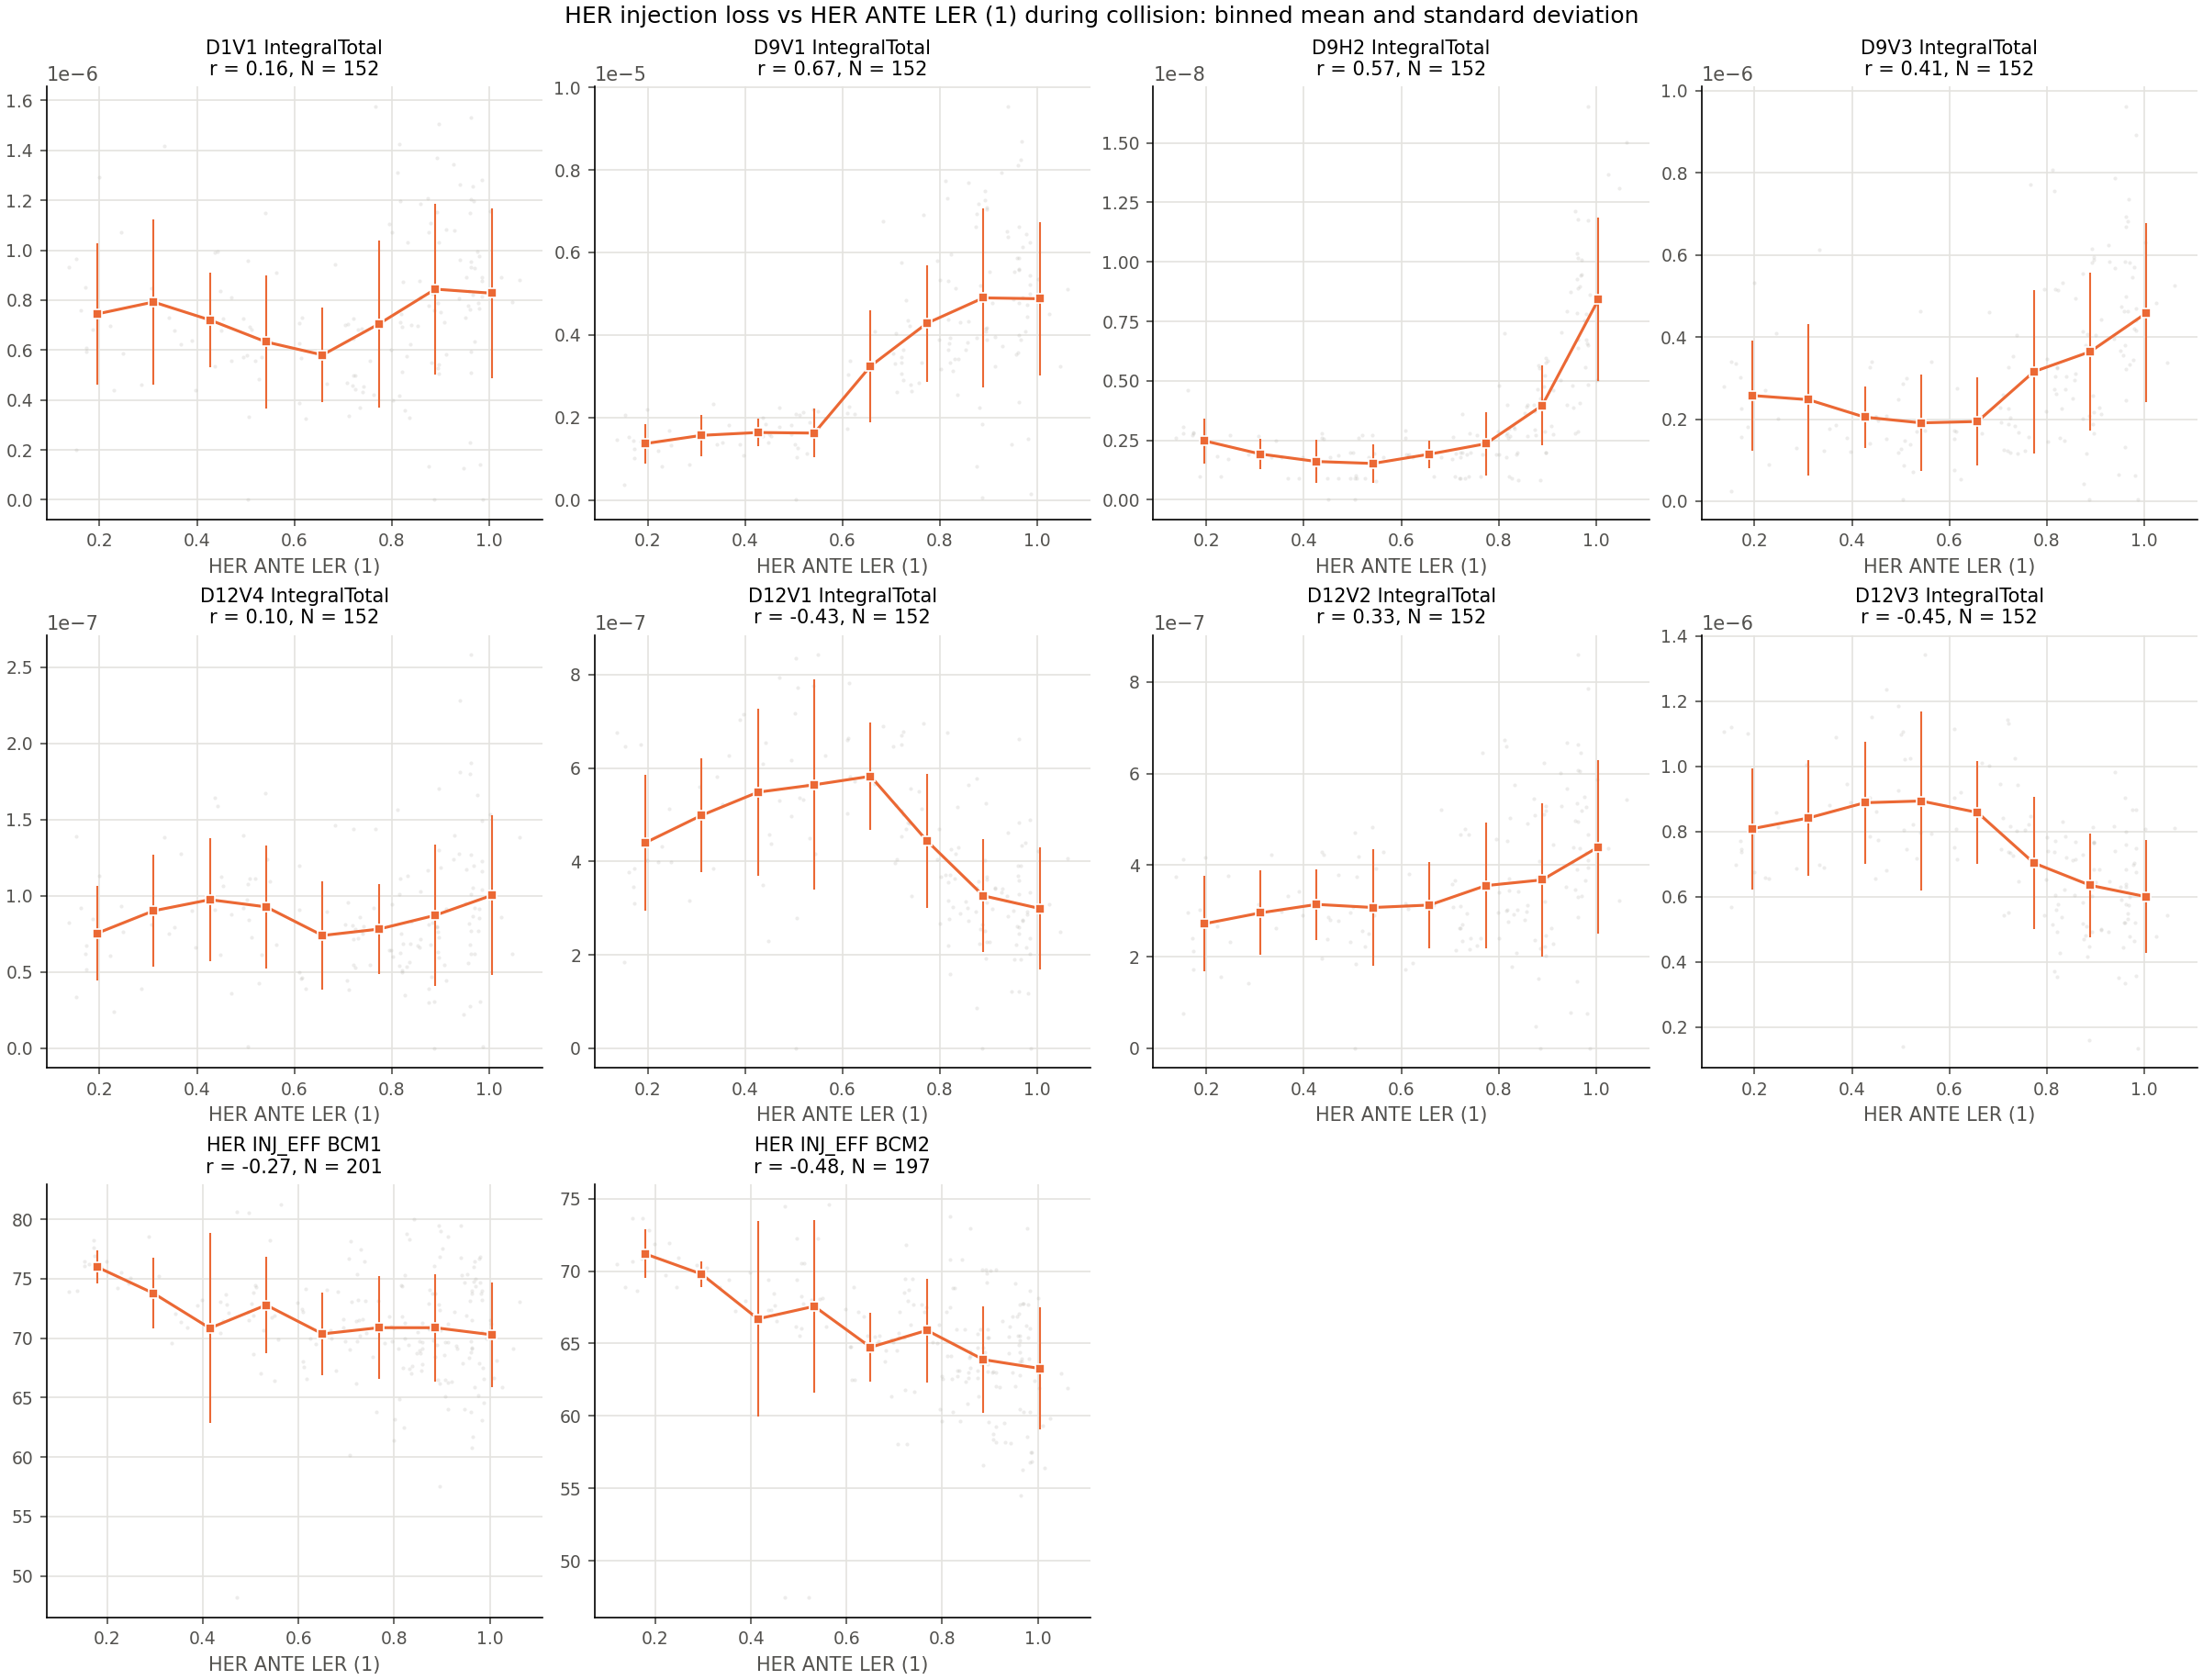
\includegraphics[width=0.8\columnwidth]{Figures/C05_Quantitative_analysis/HBCstudy/HER_ante_LER.png}
    \caption{HER injection with collision: dependence on the bunch current $\Iopp$ of the LER bunch that collides with the injected bunch.
    Upper panels: injection beam loss at each collimator.
    Lower panels: injection efficiency 1 and 2.}
    \label{fig:HER_ante_LER}
\end{figure}

Figure~\ref{fig:HER_ante_LER} shows the dependence on the colliding LER bunch current $\Iopp$.
The injection beam loss increases at D9V1 ($r = 0.67$), D9H2 ($0.57$), and D9V3 ($0.41$),
whereas it shows little correlation at D1V1 ($0.16$) and D12V4 ($0.10$), and it decreases at D12V1 ($-0.43$) and D12V3 ($-0.45$).
The dependence therefore differs among the collimators; the loss is not uniformly increasing.
The injection efficiency decreases weakly to moderately with $\Iopp$ ($r = -0.27$ and $-0.48$).


\subsection{Discussion and summary}

\paragraph{Separation of $Iinj$ and $Iopp$.}
In collision, $\Iinj$ and $\Iopp$ increase together (Fig.~\ref{fig:HBC_study_config}), so their effects cannot be separated by the plots above alone.
Single-beam data, where $\Iopp$ is absent, show the dependence on $\Iinj$ only.
The difference between the collision and single-beam dependence on $\Iinj$ is therefore a measure of the beam--beam contribution.
For example, in the LER the efficiency in collision is lower than in single beam even at low $\Iinj$, which suggests that the beam--beam effect (and not only the stored current) matters.
In addition, the beam current and the machine condition changed with time during the collision period,
so the dependence on the bunch current may partly reflect a time dependence.

\paragraph{Bend at 0.4\,mA in the LER.}
The bend of the LER injection loss and efficiency at $\Iinj \simeq 0.4$\,mA appears only with collision.
It may be related to the beginning of an instability at the start of the current accumulation, but this has not been confirmed.

\paragraph{Difference between the LER and the HER.}
The two rings show opposite trends: in the LER the injection beam loss is larger and the efficiency is lower with collision,
while in the HER the loss is larger in single beam and the efficiency is higher with collision.

\paragraph{Summary.}
\begin{itemize}
    \item In the LER, higher bunch current gives larger injection beam loss and lower injection efficiency, particularly with collision.
    The efficiency decreases strongly with the colliding HER bunch current ($r \simeq -0.85$).
    \item In the HER, the loss in single beam is larger than with collision at most collimators and increases with $\Iinj$.
    The dependence on the colliding LER bunch current differs among the collimators.
    \item $\Iinj$ and $\Iopp$ cannot be fully separated in collision with the present data.
\end{itemize}


